\RequirePackage[T1]{fontenc}
\documentclass[conference]{IEEEtran}
\usepackage{amsmath,amssymb,booktabs,graphicx,url}
\usepackage[hidelinks]{hyperref}
\begin{document}
\title{Feature Dropout for Subject-Independent Activity Recognition: Benefits and Failure Modes}
\author{\IEEEauthorblockN{Anonymous manuscript}}
\maketitle
\begin{abstract}
Missing extracted features and failed sensor axes induce different shifts in smartphone activity recognition. We evaluate weighted feature-dropout augmentation of logistic regression on subject-disjoint UCI HAR and WISDM splits, with training-only preprocessing and selection. Four classical classifiers undergo feature deletion, Gaussian perturbation, feature-family removal, and WISDM raw-axis flatlining. Across ten corruption seeds, dropout training increases macro-F1 at 50\% missing entries from 85.96\% to 87.09\% on UCI HAR and from 46.29\% to 63.50\% on WISDM. Paired subject-bootstrap intervals for these differences are [0.78,1.49] and [14.40,18.93] percentage points. A separate equal-subject analysis retains the differences after Holm correction. However, WISDM random forest slightly exceeds dropout regression at this condition, Gaussian-noise benefits do not consistently transfer, and raw-axis failures yield mixed outcomes. The findings support an inexpensive missing-feature baseline while showing why feature-space gains do not establish general sensor-failure tolerance. Code, models, predictions, and checks accompany the study; the expanded UCI analysis is exploratory.
\end{abstract}
\begin{IEEEkeywords}
pattern recognition, human activity recognition, missing features, data augmentation, subject-independent evaluation
\end{IEEEkeywords}

\section{Introduction}
Human activity recognition (HAR) maps measurements from body-worn sensors to activity classes. Its standard processing chain includes segmentation, feature extraction, and classification \cite{bulling2014}. This is a practical pattern-recognition problem: the same activity can produce different measurements across people, and a classifier must recognize patterns outside its training subjects. A second challenge is incomplete input. A missing derived statistic can be imputed with its training mean, whereas a malfunctioning accelerometer axis alters many dependent statistics simultaneously. Evaluating only random missing feature entries can conceal that distinction.

We investigate whether a simple augmentation of logistic regression provides useful robustness without requiring a GPU or a large training budget. The intervention is deliberately modest: add one independently masked copy of each standardized training example, preserve the total training weight, and train the same classifier. We compare it with clean-trained logistic regression (LR), a radial-basis-function support vector machine (RBF-SVM), and a random forest. UCI HAR supplies an established feature representation \cite{anguita2013har,uci2013har}; WISDM supplies raw accelerometer recordings from which a compact representation is extracted \cite{kwapisz2010,wisdm2012}.

The contribution is an empirical evaluation of an established robustness strategy, not a new learning algorithm. Specifically, the study provides: (i) a subject-disjoint, two-dataset comparison with training-only selection and auditable predictions; (ii) a matched-regularization ablation and an expanded regularization audit; and (iii) a direct comparison between feature-family mean imputation and raw-axis flatlining. The last comparison identifies an operational boundary of the method: improving a missing-feature benchmark does not establish tolerance to physical sensor faults.

This manuscript extends an initial UCI-only experiment. Its UCI test outcomes were already known before the expanded study, so all additional UCI analyses are treated as exploratory. The WISDM split, hyperparameter grids, and corruption conditions were recorded before fitting its models. A timestamp-cleaning amendment was made after inspecting raw-data validity and class coverage, before model evaluation. There is no external preregistration. These distinctions prevent a follow-up analysis from being presented as an untouched confirmatory experiment.

\section{Related Work}
Feature deletion has long motivated robust classification, including the adversarial formulation of Globerson and Roweis \cite{globerson2006}. Marginalized corrupted features integrate over a corruption distribution during learning \cite{vandermaaten2013corruption}. Neural-network dropout \cite{srivastava2014dropout} and its regularization analysis \cite{wager2013} provide further context. Our implementation uses one finite corrupted copy with no inverse-probability rescaling. It neither marginalizes the loss analytically nor implements the neural dropout training procedure; theoretical results for expectation-preserving dropout are not assumed to apply directly.

In HAR, dataset and evaluation choices strongly influence reported performance. UCI HAR provides engineered inertial features and a fixed subject-separated split \cite{anguita2013har}. The original WISDM study demonstrates activity recognition from cell-phone accelerometers \cite{kwapisz2010}; we use the later public v1.1 release \cite{wisdm2012}, not a reimplementation of its published experimental protocol. Work on subject cross-validation \cite{dehghani2019validation} and overlapping windows \cite{dehghani2019windows} motivates grouping by participant rather than treating adjacent windows as independent observations. Missing-sensor HAR has also been examined in a recent UCI-focused preprint \cite{saha2025missing}. Differences in preprocessing, missingness definitions, and splits prevent a direct numerical ranking against that work.

Model-selection overfitting can distort performance estimates even when the learning algorithm is unchanged \cite{cawley2010}. We therefore separate training-subject validation from held-out-subject evaluation and disclose the already-observed UCI test set. Statistical comparisons across datasets require attention to the unit of analysis \cite{demsar2006}; two datasets are insufficient to establish general algorithm superiority. Our inferential calculations concern held-out subjects within each fixed dataset, not a population of benchmark datasets.

\section{Data and Representations}
\subsection{UCI HAR}
We use all 561 released features from six activities: walking, upstairs, downstairs, sitting, standing, and laying. The official split contains 7,352 training windows from 21 subjects and 2,947 test windows from nine different subjects. The source windows span 2.56 seconds with 50\% overlap \cite{anguita2013har}. We retain the supplied representation without feature selection. Subject grouping prevents the same participant from entering both sides of a validation fold, but does not remove temporal dependence within a participant; uncertainty estimation therefore resamples subjects.

\subsection{WISDM v1.1}
We parse the original accelerometer release, whose six classes are walking, jogging, upstairs, downstairs, sitting, and standing. The released data cover 36 subjects. Records must have six valid fields, finite acceleration values, a recognized activity and subject, and a positive timestamp. Of 1,098,209 nonempty parsed records, 24,579 are rejected. Within each contiguous subject/activity recording, timestamps are stably sorted and the first occurrence of each duplicate timestamp is retained, removing 41,985 further records. Gaps exceeding one second split a recording. Windows contain 200 samples with stride 200, never cross these boundaries, and discard incomplete tails (45,045 samples). The result is 4,933 non-overlapping windows.

Sorting and deduplication were introduced after an initial strict chronology check discarded most usable windows. This amendment used timestamp validity and class counts, not model performance. It remains a preprocessing choice whose sensitivity has not been exhaustively tested. No interpolation or resampling is performed. Window durations have median 10.11 seconds and range 9.95--26.50 seconds; consequently, spectral features are expressed in cycles per sample rather than asserted to be calibrated physical frequencies.

For each of $x$, $y$, $z$, and acceleration magnitude, we calculate 12 statistics: mean, population standard deviation, minimum, maximum, median, lower and upper quartiles, mean absolute value, root mean square, mean absolute first difference, dominant non-DC Fourier bin divided by window length, and normalized spectral entropy. Three pairwise axis correlations complete the 51-dimensional vector. Constant-signal correlations are defined as zero. Using a fixed group-shuffle seed of 20261022 and a 30\% subject test fraction gives 3,125 training windows from 25 subjects and 1,808 test windows from 11 subjects. Subject IDs, class counts, window provenance, and exact feature ordering are saved in the artifact.

\begin{table}[t]
\caption{Dataset-specific representations and subject-disjoint splits.}
\label{tab:data}\centering\small
\begin{tabular}{lrr}\toprule
Property & UCI HAR & WISDM \\\midrule
Features & 561 & 51 \\
Classes & 6 & 6 \\
Train/test subjects & 21/9 & 25/11 \\
Train/test windows & 7352/2947 & 3125/1808 \\
Window overlap & 50\% & 0\% \\\bottomrule
\end{tabular}
\end{table}

\section{Methods and Evaluation}
\subsection{Weighted Feature-Dropout Training}
For feature $j$, training-only standardization gives
\begin{equation}
z_{ij}=(x_{ij}-\mu_j)/s_j,
\end{equation}
where constant features use the scaler's unit scale. Independent masks $m_{ij}\sim\operatorname{Bernoulli}(1-p)$ produce $\tilde z_i=m_i\odot z_i$. A zero standardized feature corresponds to its training mean; the mask is not rescaled. For multinomial cross-entropy $\ell$, the implemented weighted objective can be written, up to a constant factor, as
\begin{equation}
\frac{1}{2n}\sum_{i=1}^{n}\!\left[\ell(y_i,f_W(z_i))+\ell(y_i,f_W(\tilde z_i))\right]
+\frac{\lVert W\rVert_F^2}{2Cn}.
\end{equation}
Each clean and corrupted copy has sample weight 0.5, preserving total weight $n$ and the comparison at fixed $C$. The intercept is not penalized. LR uses the same preprocessing and classifier with only clean examples. Optimization uses L-BFGS, tolerance $10^{-4}$, and at most 2,000 iterations in scikit-learn \cite{pedregosa2011sklearn}. The masked copy is sampled once per fit, rather than redrawn at every optimizer step.

\subsection{Selection and Comparators}
All methods use three subject-disjoint GroupKFold partitions within training data. A separate scaler is fitted on each fold's training portion. The selection score is
\begin{equation}
S=\tfrac12\left(F_{\rm clean}+\tfrac13\sum_{r=1}^{3}F_{{\rm mask},r}(q=0.3)\right),
\end{equation}
averaged across folds. Here $F$ is six-class macro-F1 and validation corruption seeds are 101--103. Thus even clean-trained comparators are selected for the same clean/robustness objective; ``clean-trained'' does not mean ``selected only for clean accuracy.''

WISDM searches $C\in\{0.001,0.01,0.1,1,10\}$ for LR and all combinations with $p\in\{0.1,0.3,0.5\}$ for dropout LR. SVM \cite{cortes1995} uses $C\in\{1,10\}$ with scale-based kernel width. Random forest \cite{breiman2001} uses 200 trees and maximum-feature choices $\sqrt d$ or $0.2d$. These grids give 24 configurations and 72 validation fits. Selected WISDM settings are LR $C=0.1$, dropout LR $C=1,p=0.3$, SVM $C=1$, and forest feature fraction 0.2. An additional clean LR at $C=1$ isolates the augmentation effect from the selected regularization change.

The original UCI LR grid used $C\in\{0.1,1,10\}$; the follow-up adds 0.001 and 0.01 for both LR families, requiring 24 additional validation fits. The expanded audit retains $C=0.1$ for both and $p=0.1$ for dropout LR, so it does not change their test predictions. The original UCI SVM ($C=1$) and forest ($\sqrt d$) are retained. All final fits use seed 2026. The search budgets are intentionally small and unequal across families; the results compare these configurations rather than exhaustively optimized algorithms.

\subsection{Corruption Conditions}
Independent feature deletion uses $z'=m\odot z$ with missing probability $q\in\{0.1,0.3,0.5,0.7\}$. Gaussian perturbations use $z'=z+\epsilon$, with independent $\epsilon_j\sim\mathcal N(0,\sigma^2)$ and $\sigma\in\{0.1,0.3,0.5,1\}$. Ten matched seeds (901--910) are used for every stochastic condition and model. These perturbations operate after training-based standardization and do not model missing-not-at-random mechanisms.

Structured UCI tests replace all standardized features whose released names contain \texttt{Gyro}, \texttt{BodyAcc}, or \texttt{GravityAcc} with zero. These string-defined feature families are recorded explicitly and are not claimed to be a complete physical dependency graph. On WISDM, each axis group includes that axis's 12 statistics, all 12 magnitude statistics, and its two correlations (26 features). These groups overlap through derived features. Separately, a raw-axis flatline sets all 200 raw samples of one axis to zero and recomputes the entire feature vector before scaling. This latter experiment preserves the induced changes in magnitude and correlations instead of replacing their values by training means. Both interventions are synthetic stress tests, not measurements of a damaged device.

\subsection{Metrics and Uncertainty}
Macro-F1 is the unweighted mean of six class-wise F1 scores, with zero for undefined scores. We average this metric across corruption seeds, not across concatenated seed predictions. Accuracy and all per-example predictions are also saved. Five thousand paired subject-cluster bootstrap replicates resample the held-out subjects with replacement and retain every selected subject's windows. Each replicate calculates pooled macro-F1 for every fixed corruption seed and then averages those scores. Percentile 95\% intervals on paired differences preserve identical subject draws and corruption seeds across methods. They are conditional on fitted models, the subject split, and the sampled corruptions; they exclude training and split-selection variability.

A separate analysis calculates each subject's macro-F1 using only activity labels actually observed for that subject, then averages the dropout-minus-LR differences equally across subjects. An exact two-sided sign-flip test enumerates $2^9$ or $2^{11}$ sign assignments under a symmetric, exchangeable subject-difference null. Holm correction is applied to the nine clean/deletion/noise tests within each dataset. This equal-subject estimand differs from pooled macro-F1; its adjusted $p$ values must not be read as tests of the pooled-bootstrap estimand. Structured conditions and matched-$C$ analyses are exploratory and receive descriptive intervals, not a claim of family-wide significance.

\section{Results}
\subsection{Clean Recognition and Independent Missingness}
Table~\ref{tab:main} reports scores from the expanded ten-seed evaluation. On UCI HAR, SVM gives the highest clean macro-F1 (95.15\%), while dropout LR is slightly below LR (94.90\% versus 95.00\%). On WISDM, SVM again leads clean recognition (88.73\%); dropout LR reaches 86.28\% versus LR's 84.58\%. These are within-study comparisons, not cross-paper state-of-the-art claims.

\begin{table}[t]
\caption{Macro-F1 (\%). Missingness and noise scores average ten seeds.}
\label{tab:main}\centering\footnotesize
\setlength{\tabcolsep}{3pt}
\begin{tabular}{llrrrr}\toprule
Dataset & Model & Clean & $q=.3$ & $q=.5$ & $\sigma=1$ \\\midrule
UCI HAR & LR & 95.00 & 90.68 & 85.96 & 85.92 \\
UCI HAR & Dropout-LR & 94.90 & 91.33 & 87.09 & 86.53 \\
UCI HAR & RBF-SVM & 95.15 & 90.46 & 79.23 & 72.55 \\
UCI HAR & Random forest & 92.45 & 87.33 & 75.13 & 71.72 \\
WISDM & LR & 84.58 & 67.65 & 46.29 & 69.07 \\
WISDM & Dropout-LR & 86.28 & 77.60 & 63.50 & 68.41 \\
WISDM & RBF-SVM & 88.73 & 73.81 & 51.81 & 65.60 \\
WISDM & Random forest & 85.63 & 80.39 & 64.04 & 61.73 \\
\bottomrule

\end{tabular}
\end{table}

At 50\% missing entries, the pooled gain over LR is 1.13 percentage points on UCI and 17.21 points on WISDM (Table~\ref{tab:paired}). The equal-subject differences are 1.09 and 12.21 points; nine of nine UCI subjects and ten of eleven WISDM subjects improve. Their Holm-adjusted $p$ values are 0.035 and 0.018, respectively. The same corrected analysis retains differences at 30\% and 70\% missingness on both datasets, but not for clean recognition or any Gaussian-noise condition. Figure~\ref{fig:curves} shows that the benefit depends on corruption type and representation.

Dropout LR does not dominate the nonlinear baselines. On WISDM, the forest reaches 64.04\% at 50\% missingness, slightly above dropout LR's 63.50\%, and 80.39\% versus 77.60\% at 30\%. The comparison supports a useful inexpensive linear baseline, rather than the best classifier for every degraded-input setting. Relative to WISDM clean LR matched at $C=1$, the 50\%-missingness gain remains 22.16 points, with a descriptive paired interval of [19.42,23.85]. Thus the observed deletion gain is not explained solely by selecting a different $C$.

\begin{table}[t]
\caption{Dropout LR minus LR. $\Delta$ and 95\% paired subject-bootstrap intervals are pooled macro-F1 percentage points. Adjusted $p$ tests the separate equal-subject estimand.}
\label{tab:paired}\centering\footnotesize
\setlength{\tabcolsep}{3pt}
\begin{tabular}{llrrr}\toprule
Data & Condition & $\Delta$ & 95\% interval & Holm $p$ \\\midrule
UCI & Clean & -0.10 & [-0.39, +0.17] & 1.000 \\
UCI & 50\% missing & +1.13 & [+0.78, +1.49] & 0.035 \\
UCI & Noise $\sigma=1$ & +0.61 & [+0.25, +0.97] & 0.141 \\
WISDM & Clean & +1.69 & [+0.17, +3.20] & 0.129 \\
WISDM & 50\% missing & +17.21 & [+14.40, +18.93] & 0.018 \\
WISDM & Noise $\sigma=1$ & -0.65 & [-3.91, +1.21] & 1.000 \\
\bottomrule

\end{tabular}
\end{table}

\begin{figure*}[t]
\centering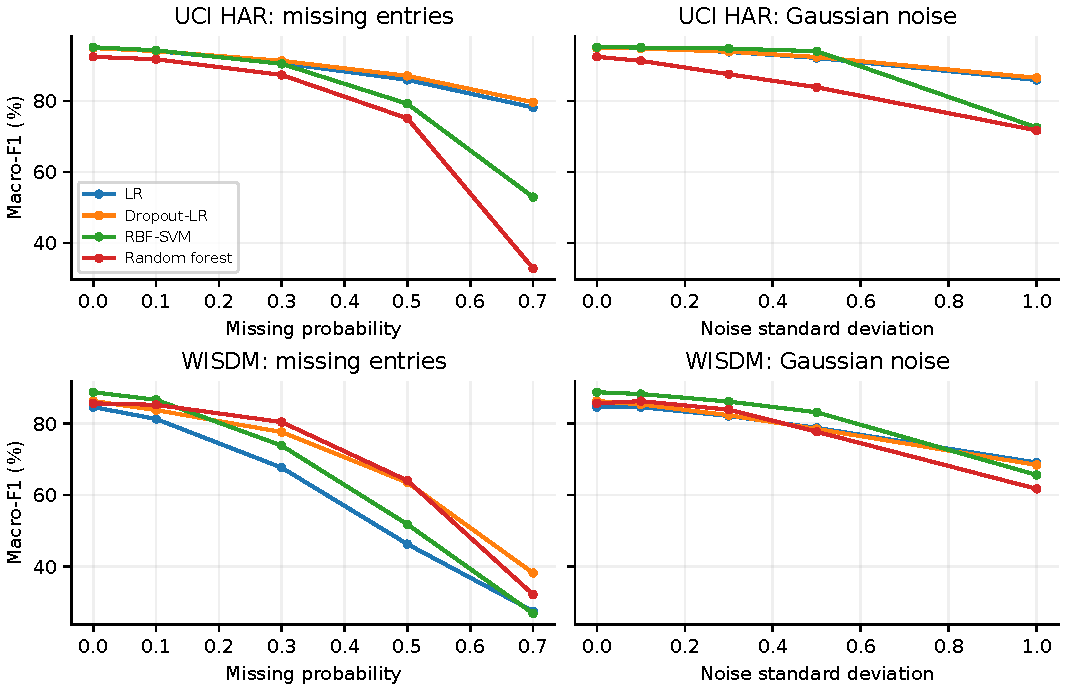
\includegraphics[width=.82\textwidth]{figures/robustness.pdf}
\caption{Macro-F1 under independent feature deletion and standardized Gaussian noise. Each nonzero point averages ten fixed corruption seeds; curves are descriptive and are not confidence bands. Representations and class sets differ between datasets.}
\label{fig:curves}
\end{figure*}

\subsection{Noise and Structured Failure}
At noise standard deviation one, dropout LR exceeds LR by 0.61 points on UCI but falls below it by 0.65 points on WISDM. The WISDM paired interval crosses zero. No Gaussian condition survives the equal-subject multiplicity correction. Deletion augmentation therefore cannot be interpreted as broadly improving additive-noise robustness.

Table~\ref{tab:structured} contrasts structured missingness with raw failures. Mean-imputing WISDM axis-dependent features produces large LR-relative gains, ranging from 11.25 to 27.41 points. Raw flatlining changes that picture: dropout LR is 0.22 points worse on the $x$ axis, 2.50 points better on $y$, and 16.71 points better on $z$. The descriptive paired intervals for these three differences are [-8.68,5.86], [-1.70,7.33], and [8.39,25.15], respectively. The $z$ result is encouraging, but the axis-specific outcomes do not justify a general sensor-failure claim. For raw $y$ failure, both linear models are below 25\% macro-F1 despite the positive difference. Absolute degraded performance matters as much as the relative improvement.

\begin{table}[t]
\caption{Structured stress tests: macro-F1 (\%) and difference in percentage points. ``Mean'' replaces the specified standardized feature family with zero; ``Raw'' recomputes features after axis flatlining.}
\label{tab:structured}\centering\footnotesize
\setlength{\tabcolsep}{3pt}
\begin{tabular}{llrrr}\toprule
Data & Intervention & LR & Dropout & $\Delta$ \\\midrule
UCI & Mean: Gyro & 82.66 & 84.46 & +1.80 \\
UCI & Mean: BodyAcc & 74.98 & 75.49 & +0.51 \\
UCI & Mean: GravityAcc & 77.97 & 81.80 & +3.83 \\
WISDM & Mean: x & 34.58 & 61.99 & +27.41 \\
WISDM & Mean: y & 37.29 & 55.95 & +18.65 \\
WISDM & Mean: z & 36.38 & 47.63 & +11.25 \\
WISDM & Raw: x flatline & 58.91 & 58.69 & -0.22 \\
WISDM & Raw: y flatline & 22.40 & 24.90 & +2.50 \\
WISDM & Raw: z flatline & 36.69 & 53.40 & +16.71 \\
\bottomrule

\end{tabular}
\end{table}

\subsection{Computation and Reproducibility}
The follow-up run completed in 232.81 seconds with numerical libraries limited to two threads on the execution host. This includes 96 new validation fits, final training, evaluation, and uncertainty calculations, but excludes initial dataset preparation and the earlier UCI experiment. WISDM final-fit times were approximately 0.06 seconds for LR, 0.17 for dropout LR, 0.10 for SVM, and 2.24 for the forest. These measurements indicate practical CPU feasibility; they are not portable latency guarantees or on-device energy measurements.

The artifact stores 504 UCI and 435 WISDM model-condition records, full prediction arrays, fold subjects, chosen parameters, and source/data checksums. Twenty-one automated checks passed, covering subject separation, saved-score recomputation, data accounting, feature dependencies, and sign-flip behavior. Manuscript tables and vector curves are generated from these CSV files. The older three-seed UCI results remain available as historical outputs; the present paper consistently reports the ten-seed follow-up. The complete project provides both training and inference code, dataset notices, and an editable IEEE LaTeX manuscript.

\section{Discussion and Limitations}
The two datasets agree that augmentation can reduce the cost of independently missing derived features. A plausible explanation is that masked training reduces reliance on individual standardized coordinates. This is an interpretation of the empirical pattern, not a proven mechanism. The much larger WISDM gain may reflect representation redundancy, feature correlations, class structure, or the selected corruption rate. Since all of these differ together, the study does not isolate which factor causes the cross-dataset gap.

Several limits constrain generalization. First, each dataset uses one train/test subject split; bootstrap intervals do not replace repeated outer subject splits. Second, corruption probabilities and severity levels are synthetic and do not model realistic fault incidence, temporal outages, drift, orientation changes, or missing-not-at-random behavior. Third, WISDM timestamp cleaning and non-resampled spectral statistics create a preprocessing dependency requiring further sensitivity analysis. Fourth, only four classical model families and modest search grids are included; deep temporal models and specialized missing-data learners are not evaluated. Fifth, the main follow-up uses one augmentation training seed. Additional seeds in the historical UCI experiment are not a substitute for multi-seed WISDM training. Sixth, only nine and eleven test subjects underpin the uncertainty estimates, and subgroup or demographic robustness is not assessed.

Stronger generalization claims require further independent datasets or repeated outer splits, preprocessing sensitivity experiments, and measured device failures. The current contribution remains an auditable evaluation of a simple baseline, not a new algorithm or a prospective deployment study.

\section{Conclusion}
Weighted feature-dropout augmentation improves subject-independent activity recognition when extracted feature entries are independently absent on two public datasets. The gains persist under a matched-$C$ comparison on WISDM and an expanded regularization audit on UCI HAR. However, clean recognition, Gaussian perturbations, nonlinear comparators, and raw-axis flatlining expose important limits. Feature-space robustness and sensor-failure tolerance should be evaluated separately. The supplied implementation makes these distinctions reproducible on a CPU without presenting an established augmentation technique as a new algorithm.

\section*{AI Assistance and Artifact Note}
An AI assistant was used for implementation, experimental scripting, literature discovery, and manuscript drafting. Reported measurements are generated by the included code and saved predictions. Human authors must review the artifact and adapt this disclosure to the selected venue before submission. Dataset ownership and original redistribution notices remain with their respective providers. No similarity-checking service or conference submission has been performed.

\bibliographystyle{IEEEtran}
\bibliography{references}
\end{document}

